\documentclass{article}

% Language setting
% Replace `english' with e.g. `spanish' to change the document language
\usepackage[english]{babel}
\usepackage[skip=2pt]{caption}

% Set page size and margins
% Replace `letterpaper' with`a4paper' for UK/EU standard size
\usepackage[letterpaper,top=2cm,bottom=2cm,left=3cm,right=3cm,marginparwidth=1.75cm]{geometry}

% Useful packages
\usepackage{amsmath}
\usepackage{graphicx}
\usepackage[colorlinks=true, allcolors=blue]{hyperref}

\title{Assignment 1}
\author{Sagar Poudel - 213051001 \\ Sejal Upadhye - 213050017}

\begin{document}
\maketitle


\section{Q1}
\subsection{(1)}
\begin{figure}[ht]
\centering
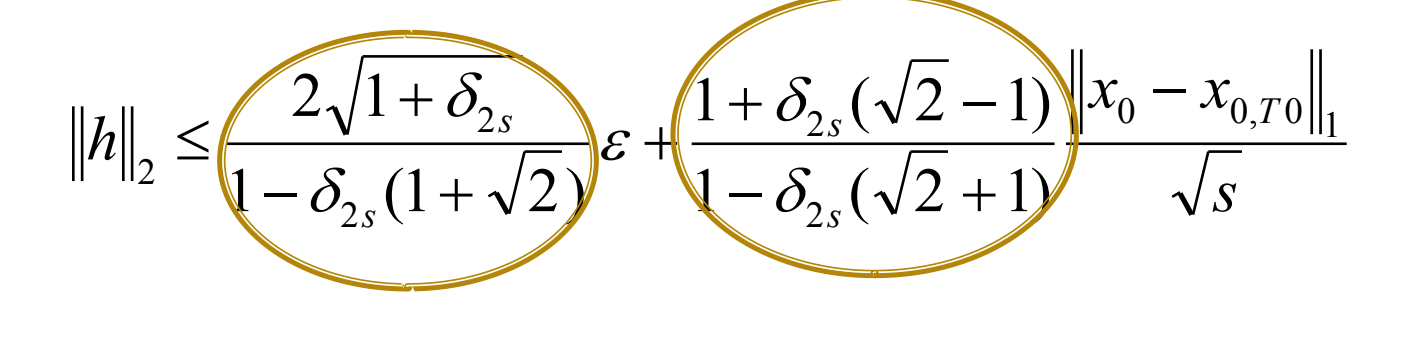
\includegraphics[width=0.5\textwidth]{c0c1.png}
\caption{Relation of $C_0$ and $C_1$ with $\delta_{2s}$}
\end{figure}
$\delta_{2s}$ is an increasing function of the sparsity of signal s. If we increase s, $\delta_{2s}$ will also increase with the constraint that $\delta_s < \delta_{s+1}$. We also know from the figure above that $C_1$ and $C_2$ are increasing functions of $\delta_{2s}$. Thus, with the increase of both the terms, we cannot surely tell whether the bound will be increased or decreased when s increases.
\subsection{(2)}
There is no direct relation of m with the given bound, but it has a few implications.\\
We know that $ O(slog(n/s) \leq m$, i.e the value of s cannot be greater than the value of n, and the value of m will have to be greater than the value of s.\\The measurement matrix has m rows. If m is less than s then the reconstruction is not possible using the above relation. Also m plays an important role in setting the value of $\epsilon$ as $\epsilon \ge 3\sigma\sqrt{m}$ for the noise measurement.
\subsection{(3)}
With the decrease in RIC value the error bound still remains the same, which we also saw in $1^{st}$ question. It is covering all the cases even if we have reduced the value of $\delta_{2s} < $ 0.1. Thus, Theorem 3 is more useful than Theorem 3A.
\subsection{(4)}
We have
$||\theta - \theta^{*}||_{2} \leq \frac{C_0}{\sqrt{S}}||\theta - \theta_{s}||_2 + C_{1} \varepsilon$.
If we set value of $\varepsilon$ = 0 in the equation, it will be similar to theorem 2. Thus our problem will be change to:
$$y = \Phi \Psi \theta$$

The model will not consider the noise value even if the noise vector $\eta$ has non zero magnitude. In every measurement there exist some noise. Thus t will over-fit the value of $\theta$ estimation.
\section{Q2}
The coherence between $m \times n$ measurement matrix $\Phi$ (with all rows normalized to unit magnitude) and $n \times n$ orthonormal representation matrix $\Psi$ must lie within the range $ [1, \sqrt{n}]$.
Coherence between $\Phi$ and $\Psi$ is given as:
$$
    \mu(\Phi, \Psi) = \sqrt{n} max_{i \in {0,1 ..... m-1}},max_{j \in {0,1 ..... n-1}} | \Phi^{i^t} \Psi_j|
$$
We know the range value lies in $[1, \sqrt{n}]$.
Lets prove the lower limit using following expression.

\textbf{$$
g = \sum^{n}_{k=1} \alpha_k \Psi_k
$$} where g is unit vector such that $g \in \mathbb{R}^n$ and $\Psi$ is an orthonormal basis.

As g is unit vector,

$$
    g^Tg = 1
$$

$$
     (\sum^{n}_{k=1} \alpha_k \Psi_k)^t  \sum^{n}_{k=1} \alpha_k \Psi_k = 1
$$

$$
     \text{Also }\sum^{n}_{k=1} \alpha_k^2=1 ,  \text{   as } \Psi \text{ is an orthonormal matrix, dot product of columns is 0 if the columns are different}
$$
Coherence between g and $\Psi$ is given as:
$$
    \mu(g, \Psi) = \sqrt{n} max_{i \in {0,1 ..... n-1}} \frac{| g^T \Psi_j|}{||g||_2 ||\Psi||_2}.
$$

As g is formed by the linear combination of $\Psi$ matrix, which is orthonormal,

$$
    \mu(g, \Psi) = \sqrt{n} max_{i \in {0,1 ..... n-1}} \frac{|\alpha_j|}{||g||_2}.
$$
Using above relation,

$$
    \mu(g, \Psi) = \sqrt{n} max_{j \in {0,1 ..... n-1}} \frac{|\alpha_j|}{||g||_2} = \sqrt{n} max_{j \in {0,1 ..... n-1}} \frac{|\alpha_j|}{\sum_{k=1}^n \alpha_k^2}  =  max_{j \in {0,1..... n-1}}   \sqrt{n} |\alpha_j |
$$
The minimum value can be achieved when all the values are same. We know g is a unit vector, if all the values are not same, hence values are normalized accordingly.

$$
g = \sum^{n}_{k=1} \alpha_k \Psi_k = n\alpha^2 = 1, \alpha ^2 = 1/n , |\alpha| = \frac{1}{\sqrt{n}}
$$
Thus, minimum value is 1 when $g = \frac{1}{\sqrt{n}}\sum^{n}_{k=1} \Psi_k$
\newline
\newline
Now for the upper bound, we will use the concept of Cauchy-Schwartz inequality
$$|xy| \le |x||y|$$

In our case:
$$|\Phi^{i^t} \Psi_t| \le |\Phi^{i^t}|| \Psi_t| $$
As values are normalized to unit magnitude,
$$|\Phi^{i^t}\Psi_t| \le |\Phi^{i^t}|| \Psi_t| \le 1$$
thus, 
$$\sqrt{n}|\Phi^{i^t} \Psi_t| \le \sqrt{n} $$
\section{Q3}
\subsection{(a)}
No, it is not possible to uniquely estimate x. As x is 1 sparse signal and $\phi$ of size 1 $\times$ n is a random measurement matrix, the signal may get lost. Likewise we don't know the exact index of the non zero-value.

If the index of the sparse signal is known, we can put the measurement value at a particular index of the measurement matrix, and determine x.
\subsection{(b)}
If  m = 2 then we have y of dimension $2 \times 1$ i.e
$$y_1 = \Phi_1j x$$
$$y_2 = \Phi_2j x$$
Looking at the above two measurements, we can say that uniqueness is not guaranteed. It might only reconstruct the unique solution in some cases. If we divide the value of output, we might get some ratio. Same ratio can be found in multiple columns, thus doesn't guarantee unique solution.
\subsection{(c)}
In this section it is known that x has only 2 non-zero elements and m=3, so we will have 3 values in our final solution:
$$y1 = \Phi_{1i} * x_i + \Phi_{1j} * x_j , y2 = \Phi_{2i} * x_i + \Phi_{2j} * x_j, y3 = \Phi_{3i} * x_i + \Phi_{3j} * x_j$$

We also know that for s sparse vector, there must be 2s columns to be linearly independent.
We can see that the dimension of the measurement is 3, so 4 measurement vectors in 3 dimensions implies that the vectors will be linearly dependent.
We know that in our case for 2 sparse vector we need 4 columns to be independent, but in the given dimensions, this is not possible.
\newline
Thus, no such instance of $\Phi$ is present where x can be uniquely estimated.
\subsection{(d)}
When x is 2s sparse and four measurements are taken, it is quite possible.
We know that for s sparse column, there must be 2s columns to be linearly independent.
As there will be four measurements, it is possible that x can be uniquely estimated. 
\section{Q4}
We are given two problems here in the question:
\newline
P1: Minimize $||x||_1$ w.r.t. x such that $||y − Ax||_2  \le e$
\newline
Q1: Minimize $||Ax - y||_2 $ w.r.t  x with constraint $||x||_1 \le t$

To prove:
If x is a unique minimizer of P1 for some value e $\ge$ 0, then there exists some value t $\ge$ 0 for which x is also a unique minimizer of Q1.

Proof:
Consider x is a unique minimizer of P1.
Using the hint given,
z is some vector whose L1 norm is less than t. Given t = $||x||_1$
then, $$||z||_1 \le  ||x||_1$$

Then for the solution of Q1:
$||Az - y||_2 \le ||Ax-y||_2$.
As we have minimized the solution for Q1 with $||z||_1 \le ||x||_1$ 
let us check the same for P1,

As the L1 norm of z is less than x, we have new solution,
$$||y - Az||_2 \le e$$

We already have x as unique solution for P1.
Let us say if the norm of both vector is same but values are different, then there exist two solutions which will break unique solution constraint.

Thus z = x.
\section{Q5}
\subsection{(a)}
Lists are easy to create:
\begin{itemize}
  \item Name: A Compressed Sensing-Based Wearable Sensor
Network for Quantitative Assessment of
Stroke Patients
  \item Authors: Lei Yu, Daxi Xiong, Liquan Guo and Jiping Wang
  \item Journels and Publication: Sensors 16, no. 2 (2016): 202.
  \item Link: https://www.mdpi.com/1424-8220/16/2/202
\end{itemize}
\subsection{(b)}
Stroke, also known as a cerebrovascular insult or brain attack, is when poor blood flow to the brain results in cell death. There is an increase of stroke patients every year, but there is a limited number of rehabilitation centers/resources. It is difficult for stroke patients to do rehabilitation training in a home setting. With the development of IoT, wearable devices have been widely applied in the health sector. Considering sensors like inertial measurement sensors such as accelerometers, gyroscopes and magnetometers are used to monitor and analyze the motor function of stroke patients. These sensor data were wirelessly transmitted from devices to a receiver using the ZigBee protocol. The battery life is inversely proportional to the amount of data. Hence to extend the battery life and reduce the amount of data during sampling and transmission, Lei et al. proposed compressed sensing wearable sensor device.
\begin{figure}[ht]
\centering
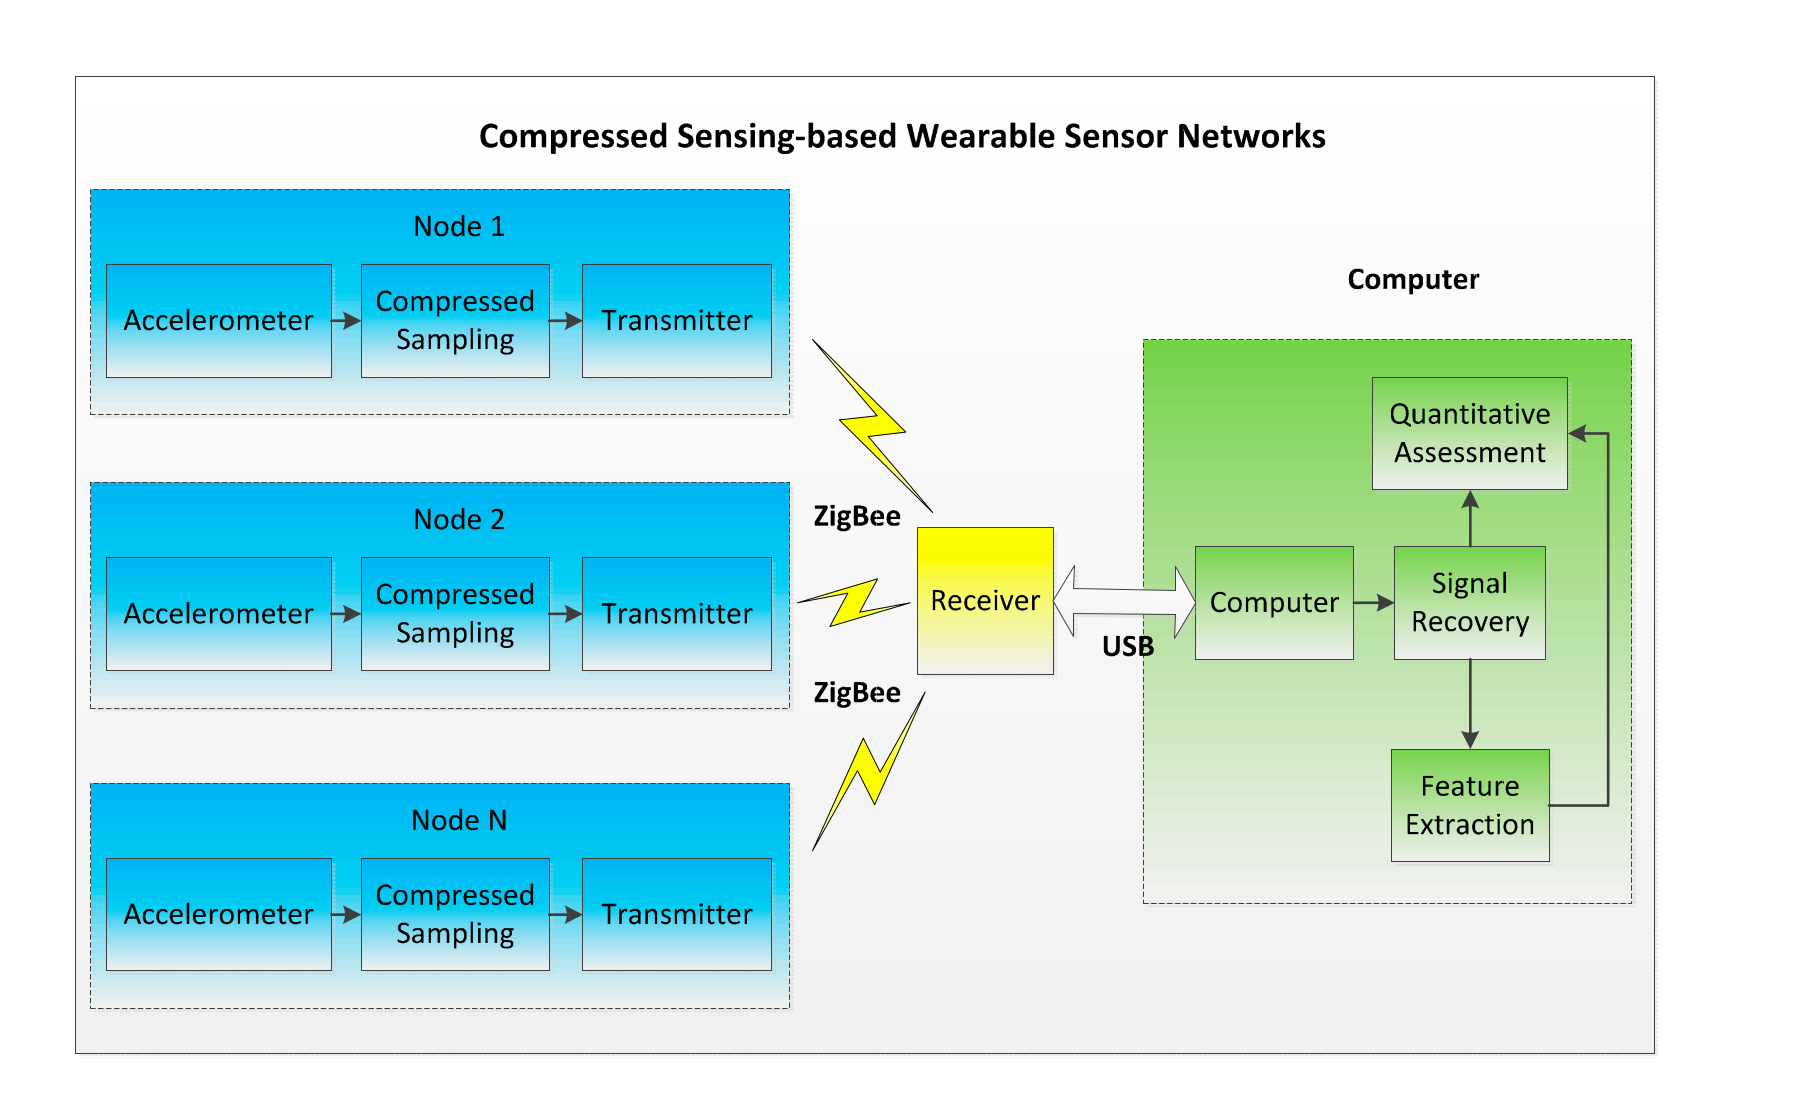
\includegraphics[width=.8\textwidth]{papers/archietecture.png}
\caption{System structure of a compressed sensing-based wearable sensor network}
\end{figure}
The compressed sensing-based wearable sensor network consists of three components: a sensor node, ZigBee wireless receiver, and a computer.  In the sensor node through compressed sampling, the sampling rate was reduced and the transmission processes were much lower. The ZigBee wireless receiver receives the data and sends it to the computer to reconstruct the signals.

\subsection{(c)}
For compressive reconstruction, the paper used the following solution:
$$
    y = \Phi x + v
$$
where , $x \in \mathbb{R}^{N \times 1}$ is a part of raw accelerometer signal,  $y \in \mathbb{R}^{M \times 1}$ is the compressed data that will be wirelessly transmitted to the server, $ \Phi \in \mathbb{R}^{M \times N }(M << N)$ is a designed sensing matrix. The model used in this paper is a noiseless model, expressed as:
$$y = \Phi x$$
X was sparse under a certain orthogonal space $\Psi \in \mathbb{R} ^{N \times N}$, thus x can be represented as:
$$ x = \Psi \theta $$
For the ease of hardware implementation, the sparse Gaussian random matrix was adopted, where the value of every element was previously embedded into the micro controller unit.

L1 norm optimization solution is used.
$$ min||\theta||_1 s.t. y = \Phi \Psi \theta$$ 
Traditional reconstruction algorithm like BP, OMP were used but didn't get expected result. Considering the signal generally has block/group structure and there exist intra-block correlation among the elements within each block, Block SBL(BSBL) algorithm gave the expected result.
\begin{figure}[ht]
\centering
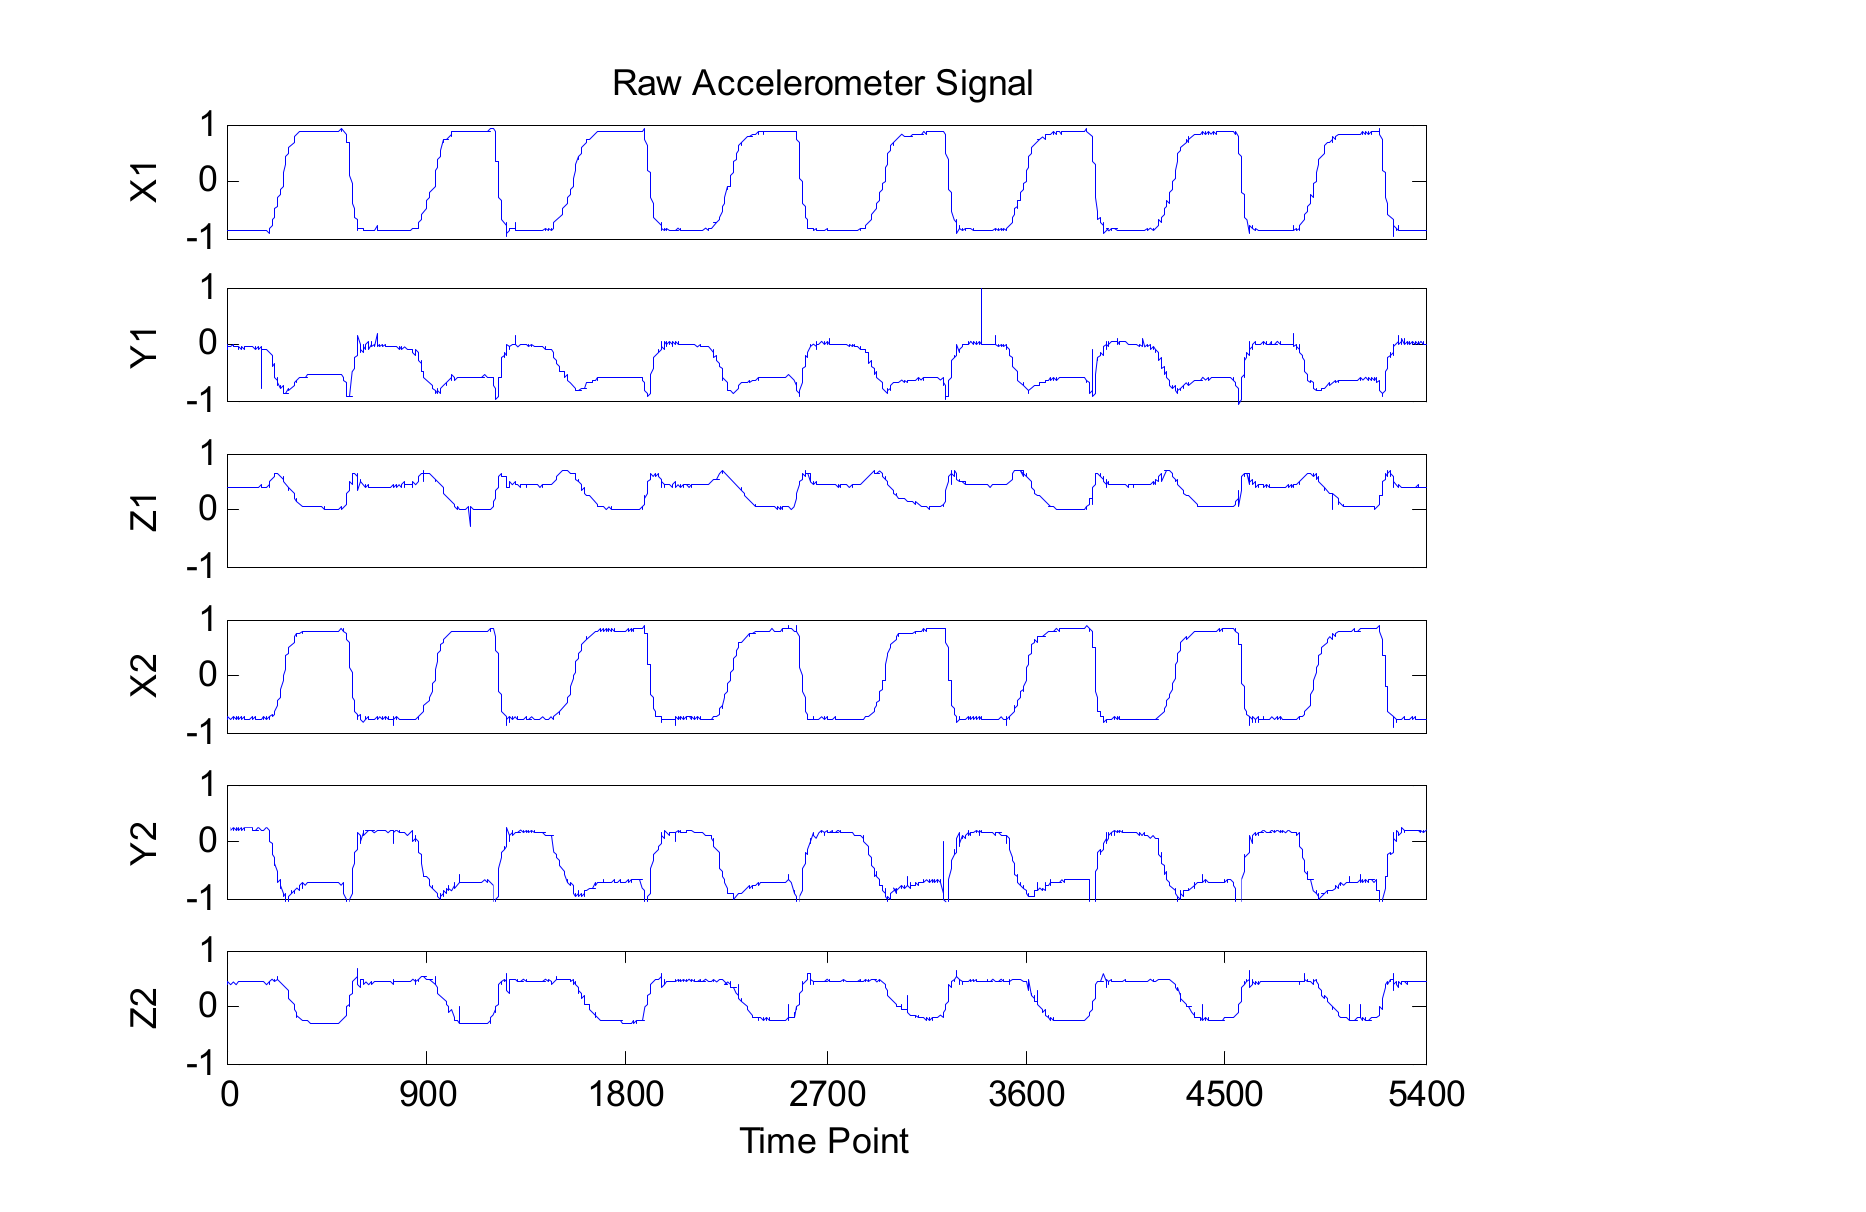
\includegraphics[width=.8\textwidth]{papers/raw_signals.png}
\caption{Raw accelerometer signals}
\end{figure}
The raw signal from exercise is shown in the above figure. The sensor shows period changes. 5400 raw sampling data in each axis needs to be transmitted to the server.
As mentioned above by adjusting the dimension of $\Phi$, the compression ratio CR is given as:

$$ CR = \frac{N-M}{N} = 1 - \frac{M}{N}$$
First, the CR was set to 0.722. This means raw sample was reduced to 1500 sampling data. The below figure shows compressed signal due to randomness of $\Phi$ and reconstructed signal using BSBL algorithm.

\begin{figure}[ht]
\centering
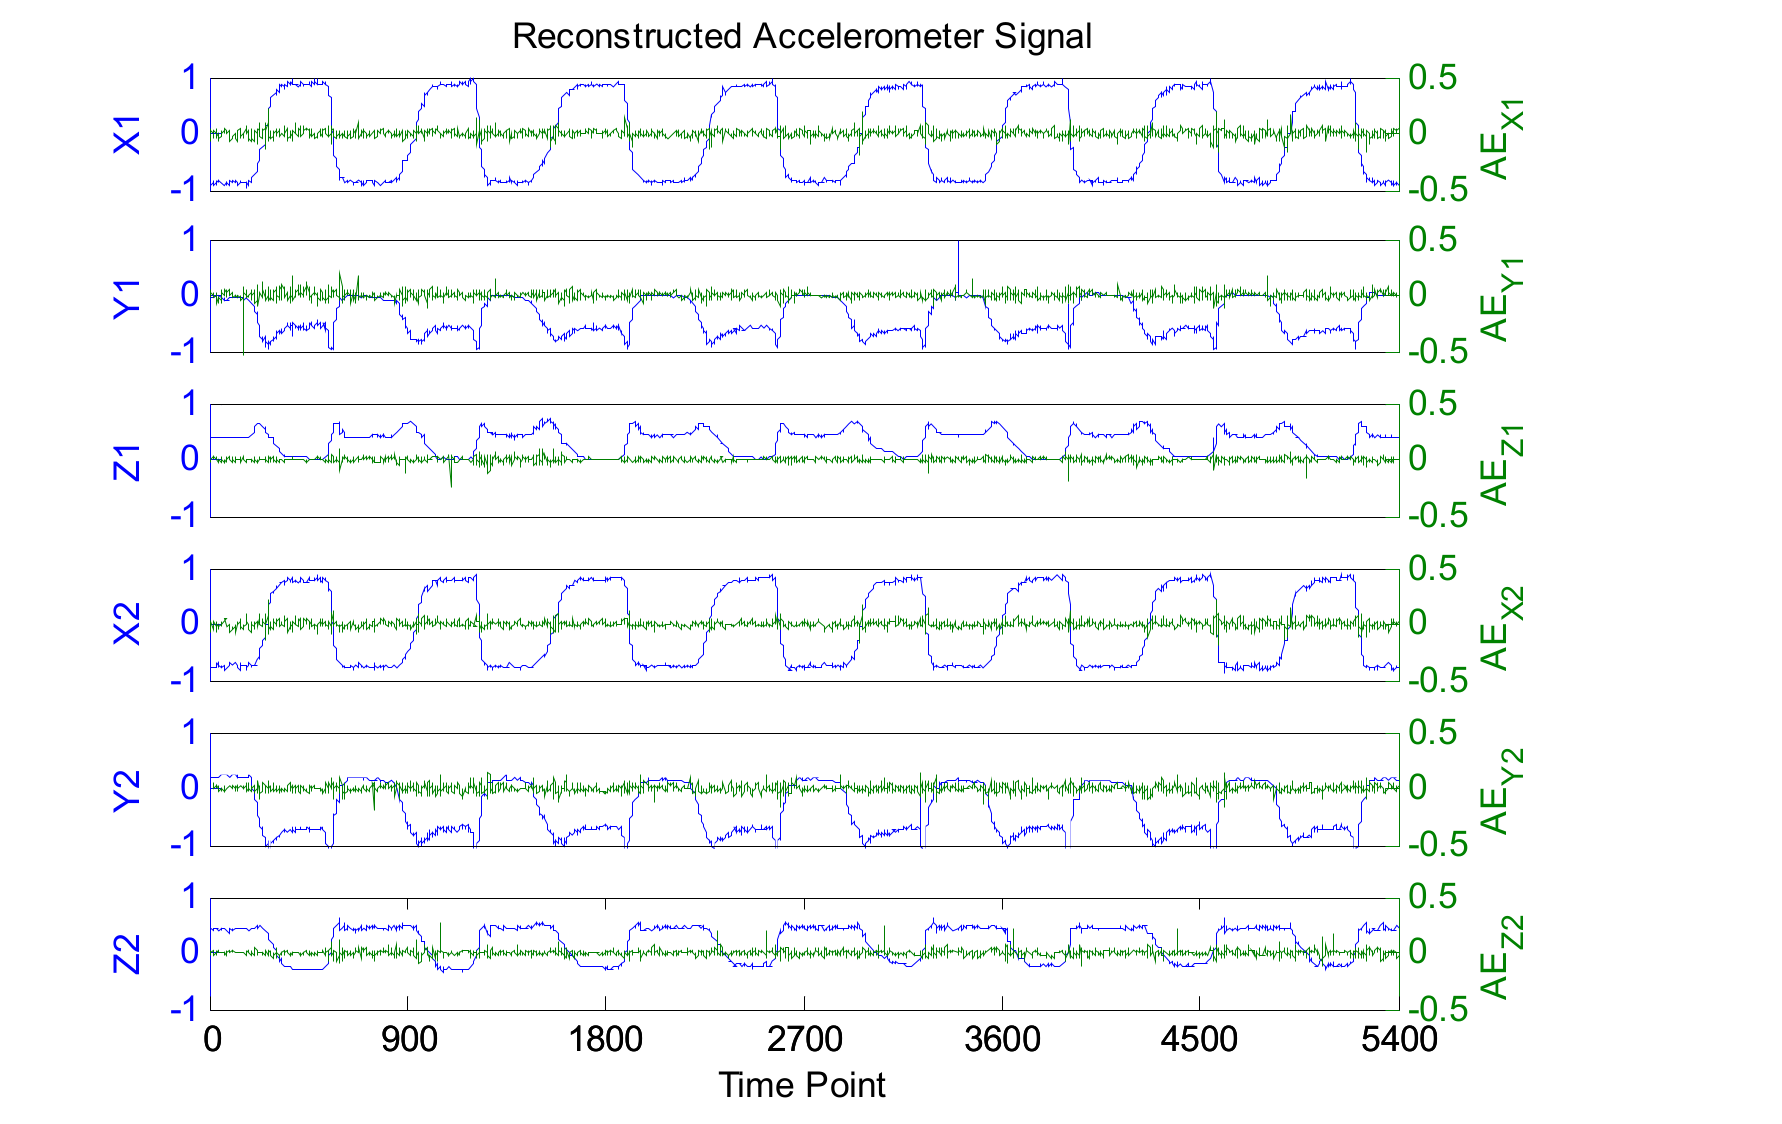
\includegraphics[width=0.8\textwidth]{papers/result.png}
\caption{Reconstructed signal(Blue), compressed signal(Green)}
\end{figure}
\newpage
\section{Q6}
\subsection{(a)}
The first three frames extracted from the video in grayscale format are as follows:
\begin{figure}[ht]
\centering
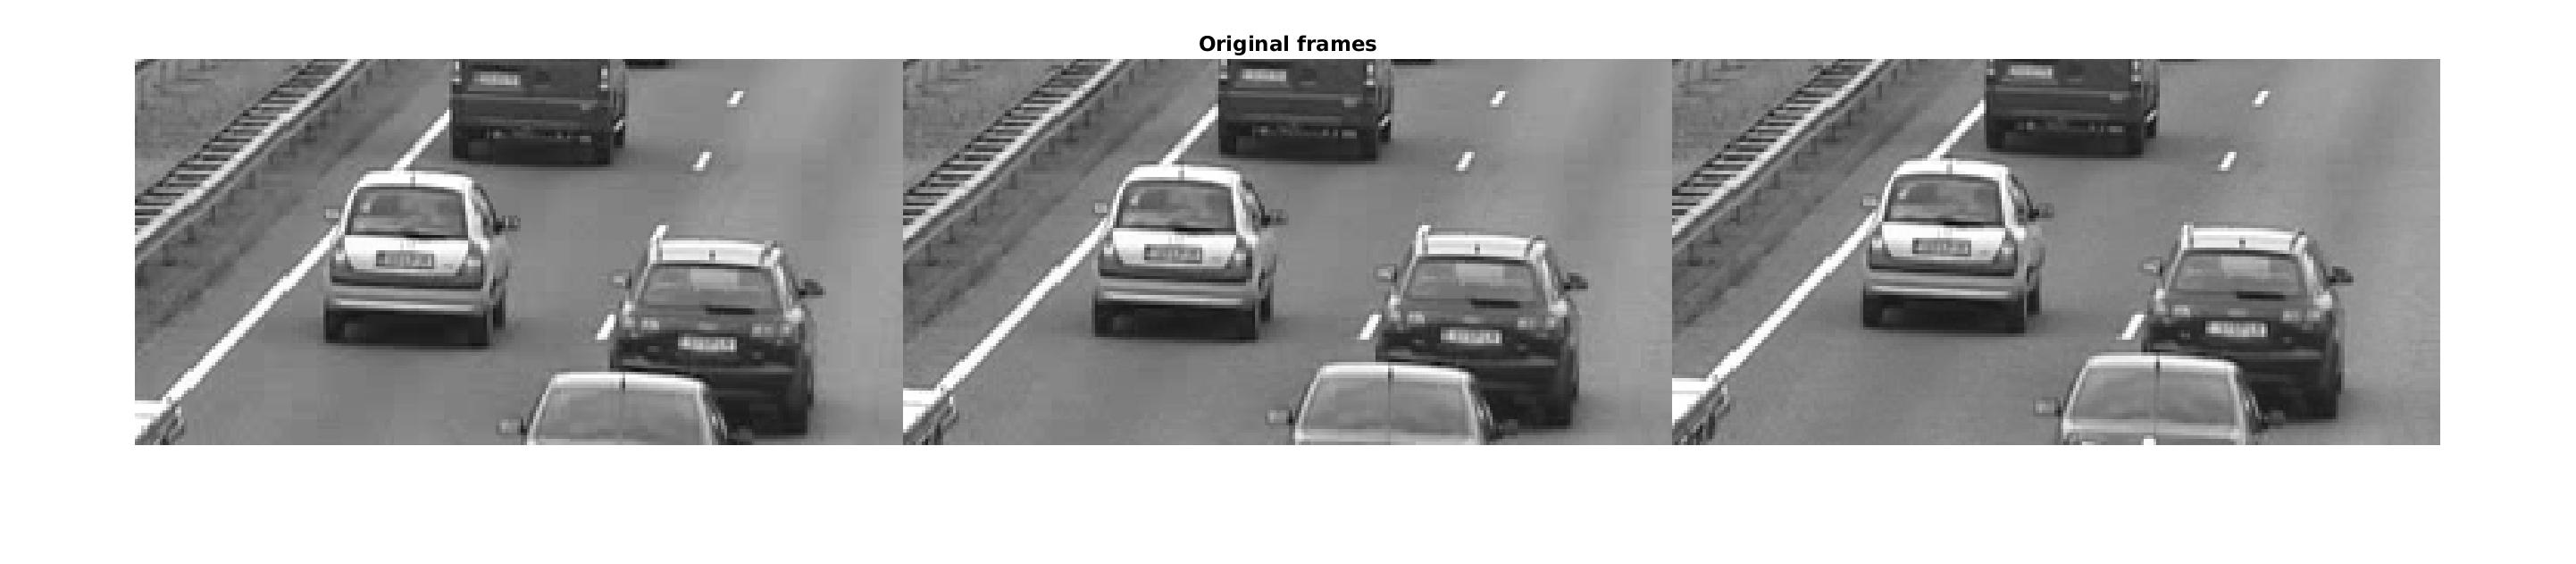
\includegraphics[width=1\textwidth]{t3/all.jpg}
\caption{T = 3 extracted frames}
\end{figure}

\subsection{(b)}
The coded snapshot for T = 3 is:
\begin{figure}[!h]
\centering
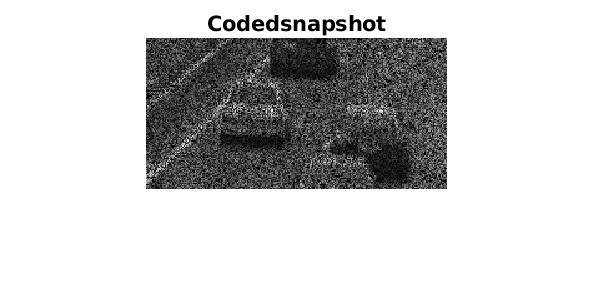
\includegraphics[width=1\textwidth]{t3/codedsnapshot.jpg}
\caption{Coded Snapshot for T = 3}
\end{figure}

\newpage
\subsection{(c)}

\begin{equation}
    \emph E_u = \Sigma^T_{t=1} C_{t} . F_t
\end{equation}
Rewriting the equation in the form of,
$$ \mathbf{ b = A  x}$$
$$b = \text{Vectorized } E_u \in \mathbb{R}^{HW}$$
$$x = \text{Vectorized } F_u \in \mathbb{R}^{HWT}$$
$$A = [S_1|S_2|\cdots|S_T], S_t = \text{diag}(C_t(:)) \in \mathbb{R}^{HW \times HWT}$$

\subsection{(d)}
Rewriting the above equation in below format: 
$$ \mathbf{Ax = b}$$
$$A = \Phi \Psi \in \mathbb{R}^{64\times64T} $$
$$\Phi =  [ S_{i1}| S_{i2}|.....| S_{iT}], S_{it} = diag(C_{it} (:)) \In \mathbb{R} ^{64x64T}$$
$$\Psi = I_T \Psi_{64, 64}]$$
$$\psi_n = \text{2D DCT Basis matrix of size n}\times \text{n}$$
$$x \in \mathbb{R}^{64T} ,  \text{sparse}$$
$$b \in \mathbb{R}^{64}$$

In this above experiment value of $\epsilon$ was set to 0.035. We have used the im2double() function, where the values are normalized in range [0,1]. We have set value of $\epsilon = 9*4*64$ and normalized with 255 for im2double.

Referring to lecture 6:
The value of $\epsilon$ depends on the noise distribution, and given the magnitude of noise will lie within 3 sd from the mean, 
i.e set $$  \epsilon \ge 3 \sigma \sqrt{m}$$
In the above experiment, we have squared the value and found the value of epsilon.
$$9*4*64 = 2304 = 0.035(\text{Normalized to} [0,1]\text{, using im2double}), \sigma = 2, m = 64 \text{ for each patch}$$

\newpage
\subsection{(e)}
For T = 3, the relative mean error is: 0.0110 below are the reconstructed images
\begin{figure}[!htb]
\centering
\includegraphics[width=1\textwidth]{t3/t1.jpg}
\caption{t = 1 Reconstructed Image: Left | Original Image: Right}
\end{figure}
\begin{figure}[!htb]
\centering
\includegraphics[width=1\textwidth]{t3/t2.jpg}
\caption{t = 2 Reconstructed Image: Left | Original Image: Right}
\end{figure}
\begin{figure}[!htb]
\centering
\includegraphics[width=1\textwidth]{t3/t3.jpg}
\caption{t = 3  Reconstructed Image: Left | Original Image: Right}
\end{figure}


\newpage
\subsection{(f)}
For T = 5 the relative mean error is : 0.019
\begin{figure}[!htb]
\centering
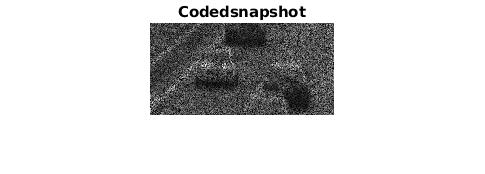
\includegraphics[width=1\textwidth]{t7/coded.jpg}
\caption{Coded Snapshot for T = 5}
\end{figure}
\begin{figure}[!htb]
	\centering
	\begin{minipage}[bt]{0.4\linewidth}
		\centering
			\includegraphics[scale=0.07]{t5/t1.jpg}
			\caption{$t = 1$}
			\includegraphics[scale=0.07]{t5/t2.jpg}
			\caption{$t = 2$}
			\includegraphics[scale=0.07]{t5/t3.jpg}
			\caption{$t = 3$}
	\end{minipage}
\begin{minipage}[!htb]{0.5\linewidth}
\centering
	\includegraphics[scale=0.06]{t5/t4.jpg}
	\caption{$t = 4$}
	\includegraphics[scale=0.06]{t5/t5.jpg}
	\caption{$t = 5$}
\end{minipage}
\caption{T = 5  Reconstructed Image: Left | Original Image: Right}
\end{figure}

\newpage
For T = 7 the relative mean error is : 0.032
\begin{figure}[!htb]
\centering
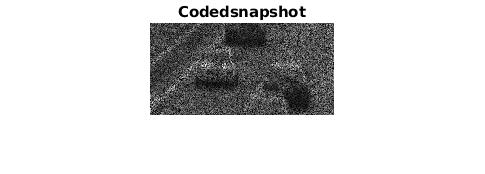
\includegraphics[width=1\textwidth]{t7/coded.jpg}
\caption{Coded Snapshot for T = 7}
\end{figure}
\begin{figure}[!htb]
	\centering
	\begin{minipage}[!htb]{0.4\linewidth}
		\centering
			\includegraphics[scale=0.07]{t7/t1.jpg}
			\caption{$t = 1$}
			\includegraphics[scale=0.07]{t7/t2.jpg}
			\caption{$t = 2$}
			\includegraphics[scale=0.07]{t7/t3.jpg}
			\caption{$t = 3$}
			\includegraphics[scale=0.07]{t7/t4.jpg}
			\caption{$t = 4$}
	\end{minipage}
\begin{minipage}[!htb]{0.5\linewidth}
\centering
	\includegraphics[scale=0.06]{t7/t5.jpg}
	\caption{$t = 5$}
	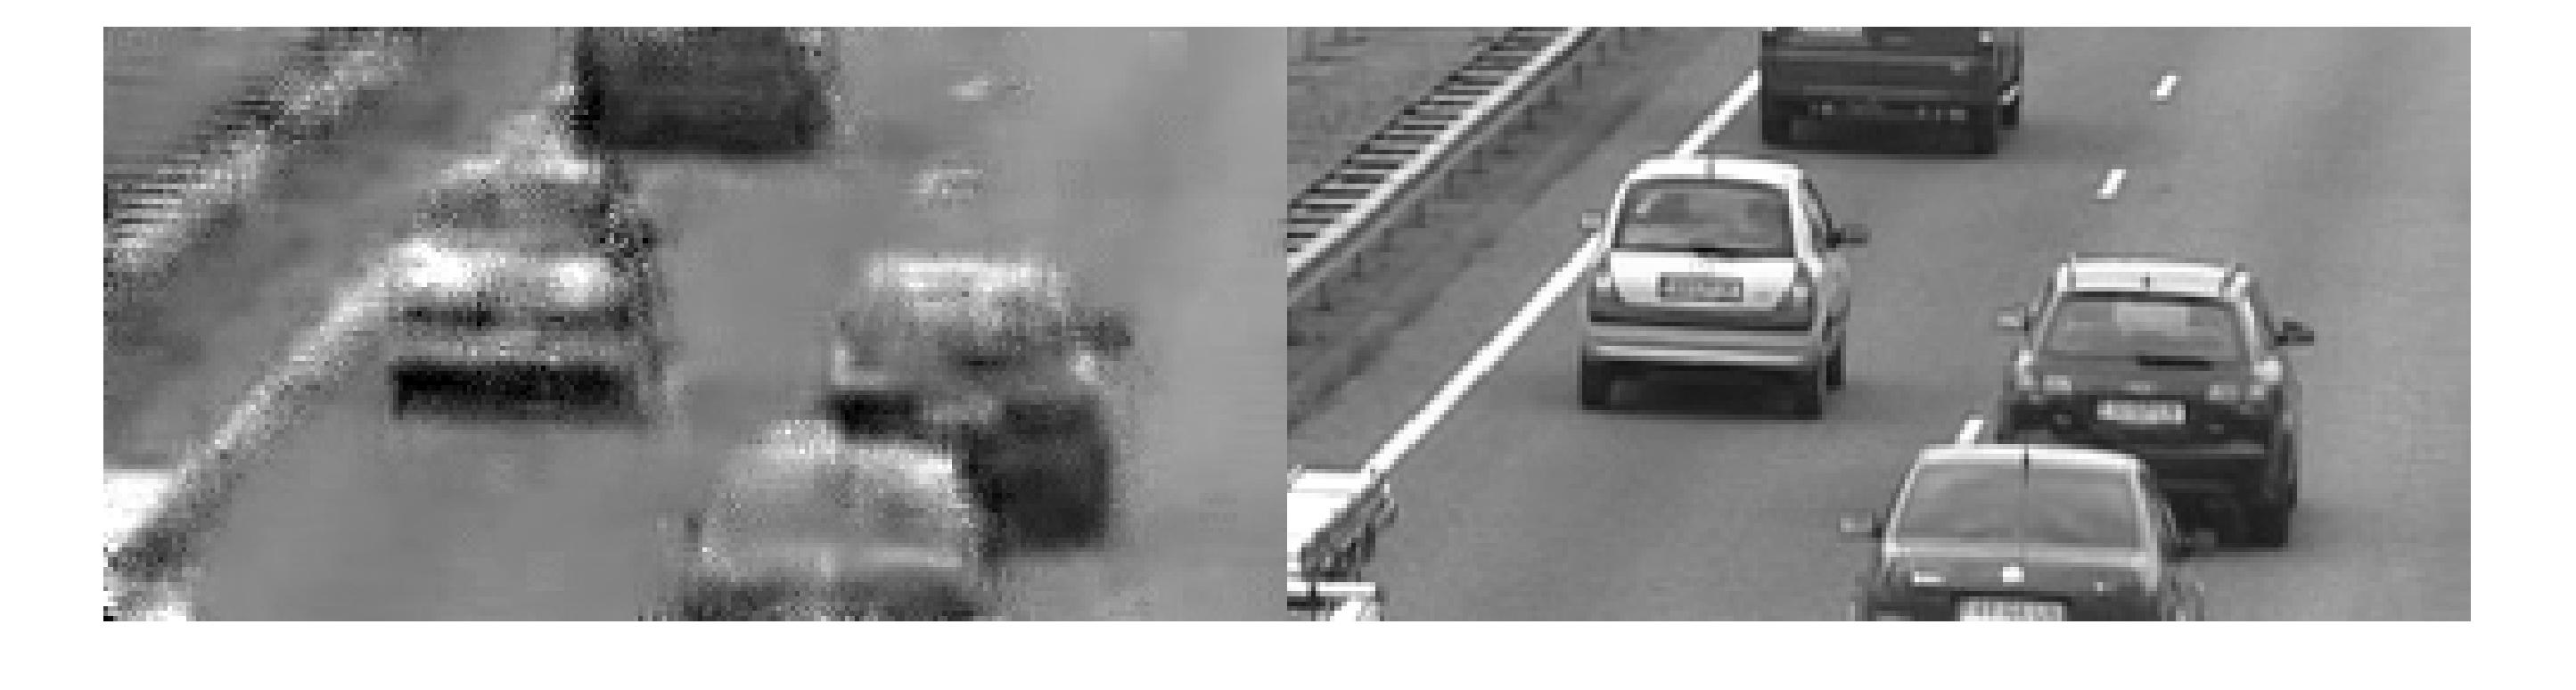
\includegraphics[scale=0.06]{t7/t6.jpg}
	\caption{$t = 6$}
	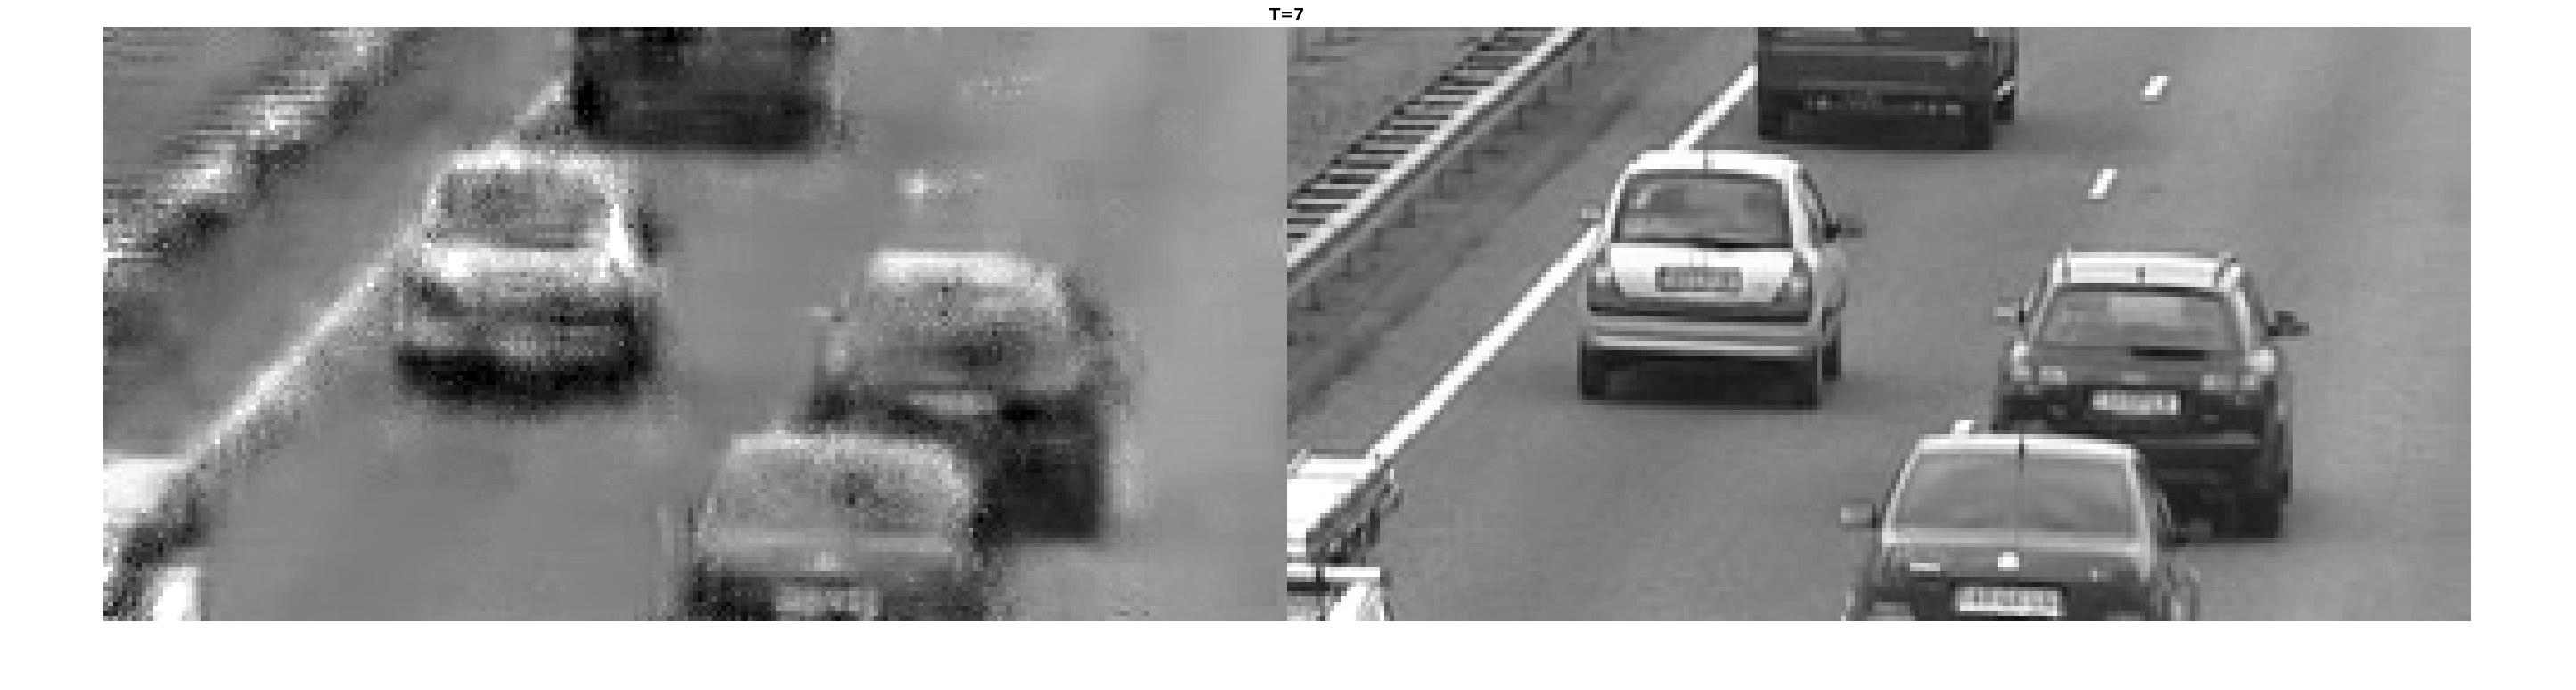
\includegraphics[scale=0.06]{t7/t7.jpg}
	\caption{$t = 7$}
\end{minipage}
\caption{T = 7  Reconstructed Image: Left | Original Image: Right}
\end{figure}

\newpage
\subsection{(g)}
To save time, extract a portion of about 120 × 240 around the lowermost car in the cars video and work entirely with it.
\subsection{(h)}
The relative mean square of 'flame.avi' video is: 
\begin{figure}[ht]
\centering
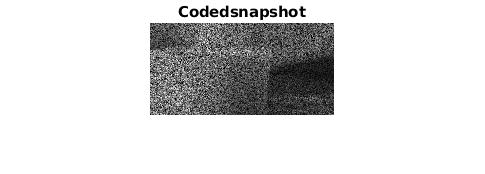
\includegraphics[width=1\textwidth]{flame/coded.jpg}
\caption{Coded Snapshot for T = 5 for flame.avi video}
\end{figure}
For T = 5 the relative mean error is : 0.001
\begin{figure}[ht]
	\centering
	\begin{minipage}[!htb]{0.4\linewidth}
		\centering
			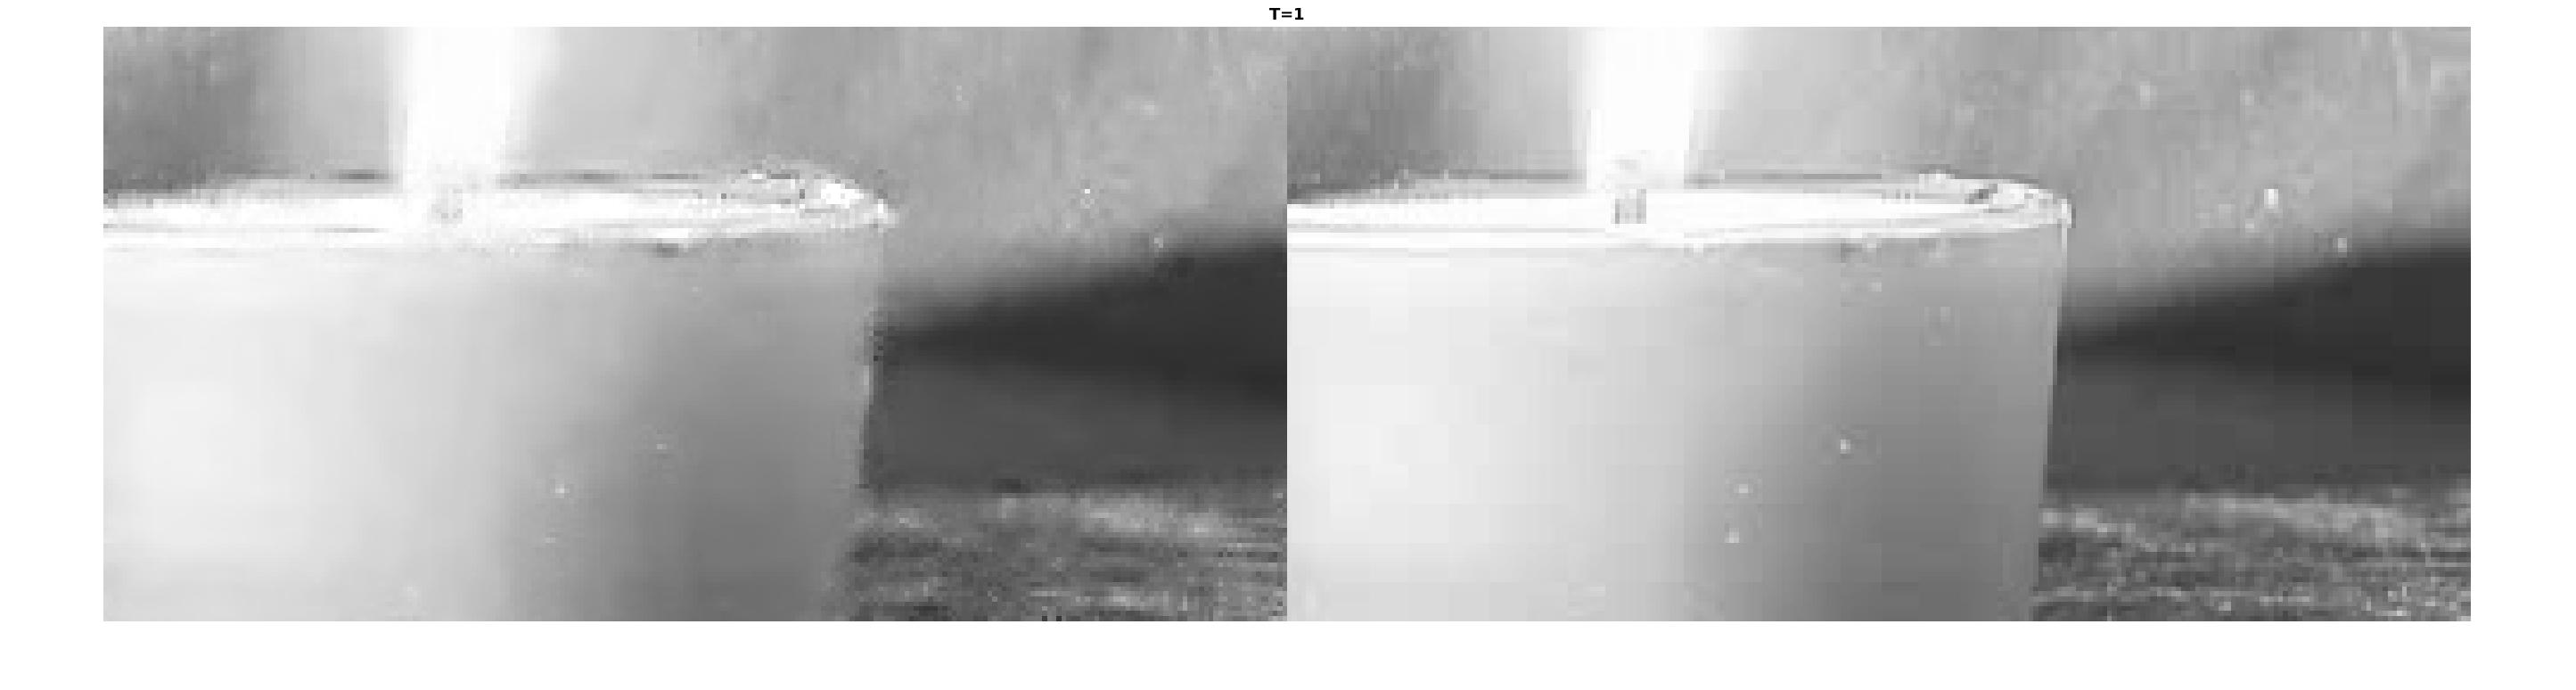
\includegraphics[scale=0.07]{flame/t1.jpg}
			\caption{$t = 1$}
			\includegraphics[scale=0.07]{flame/t2.jpg}
			\caption{$t = 2$}
			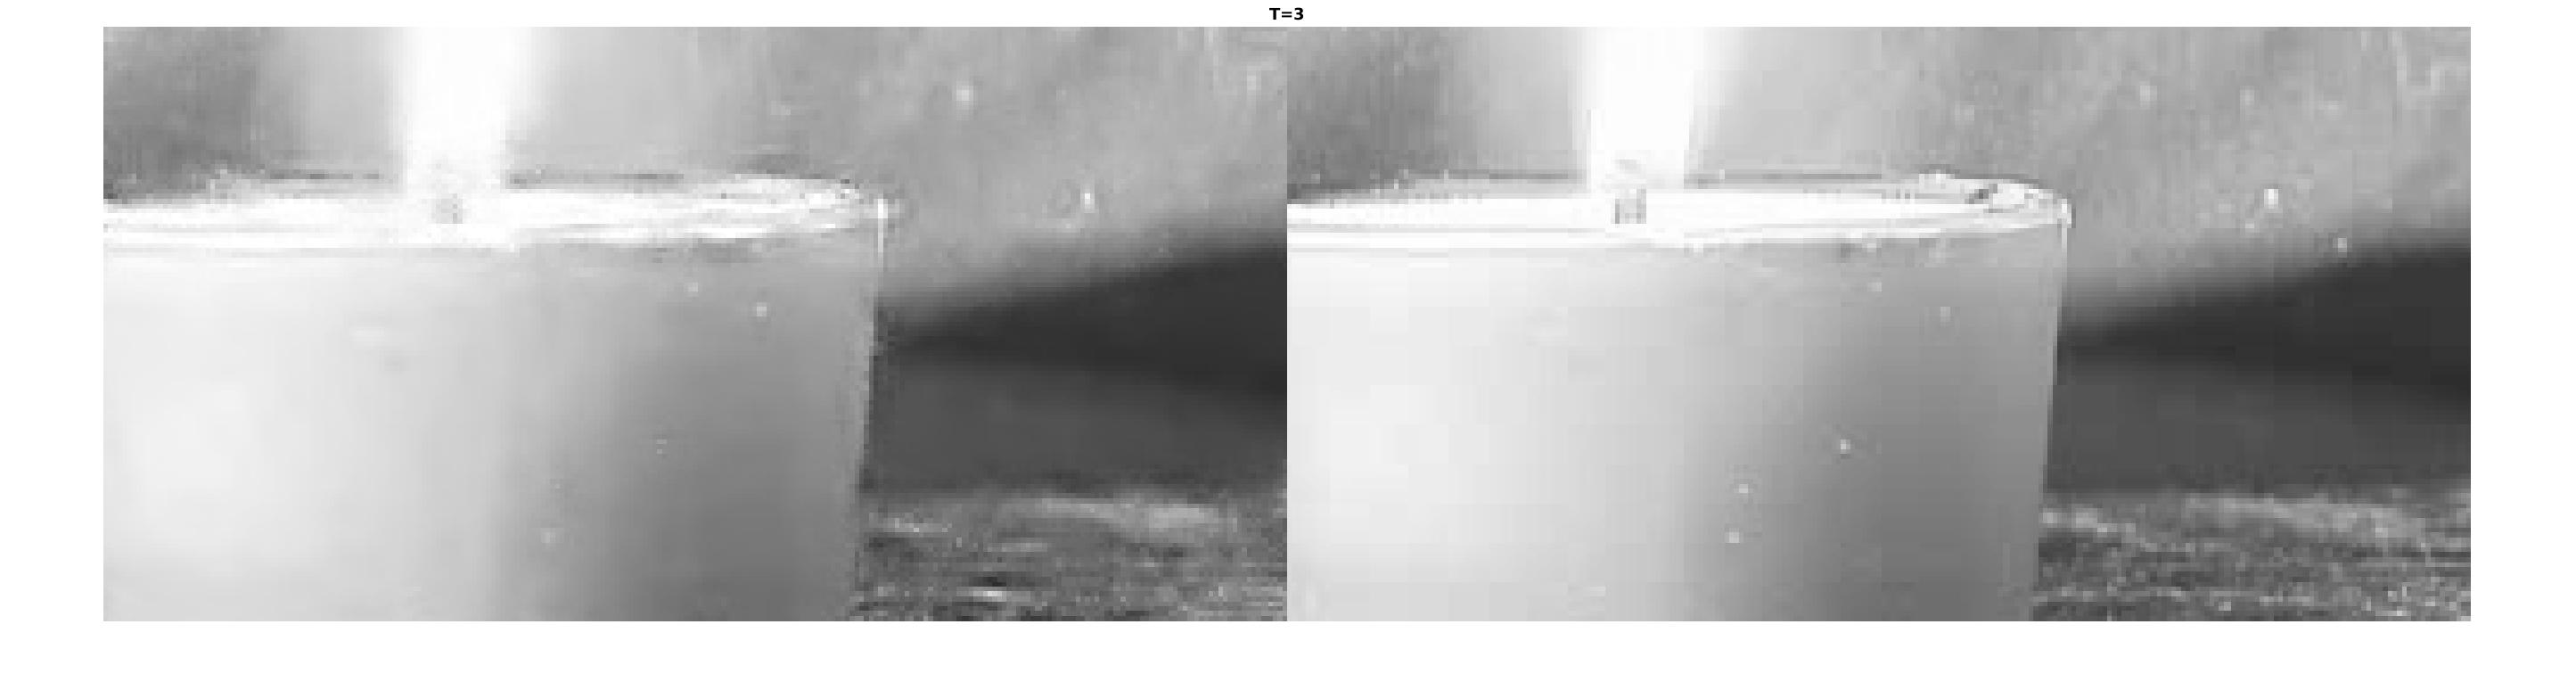
\includegraphics[scale=0.07]{flame/t3.jpg}
			\caption{$t = 3$}
	\end{minipage}
\begin{minipage}[!htb]{0.5\linewidth}
\centering
	\includegraphics[scale=0.06]{flame/t4.jpg}
	\caption{$t = 4$}
	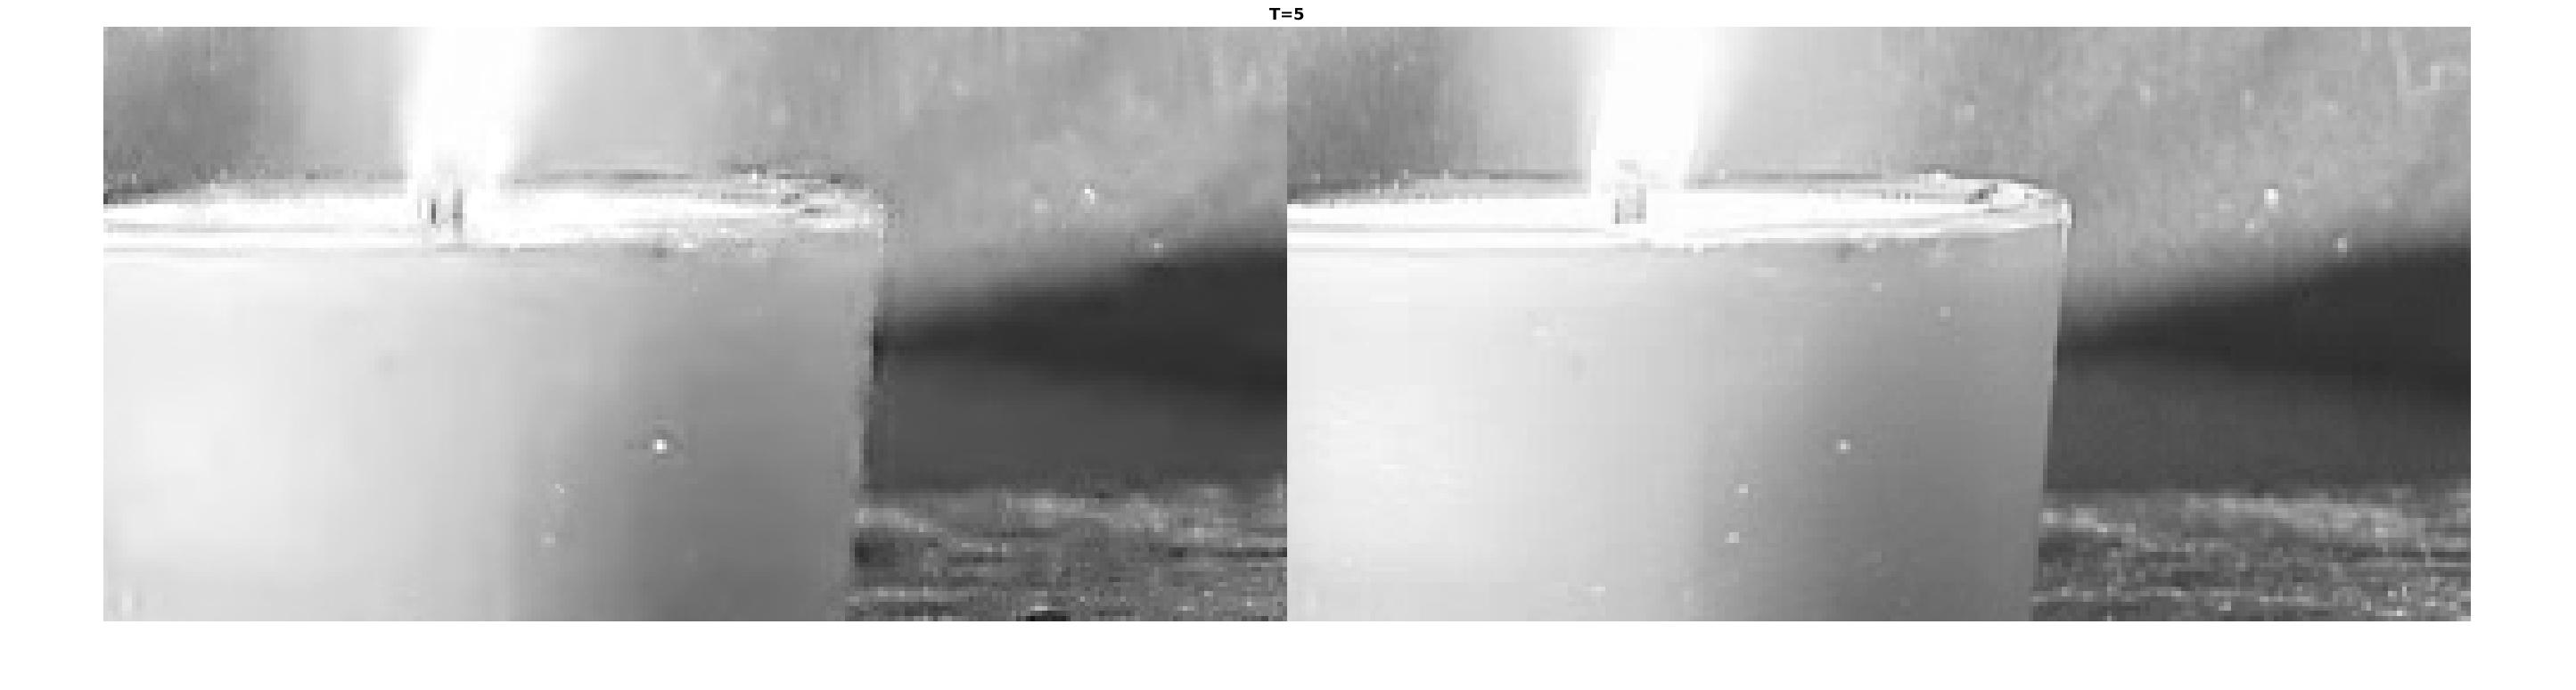
\includegraphics[scale=0.06]{flame/t5.jpg}
	\caption{$t = 5$}
\end{minipage}
\caption{Flame image: T = 5  Reconstructed Image: Left | Original Image: Right}
\end{figure}

\end{document}

